\documentclass[12pt]{article}
\usepackage[frenchb]{babel}
\usepackage[T1]{fontenc}
\usepackage{graphicx}
\usepackage[utf8]{inputenc}
\usepackage{hyperref}
\usepackage{tango}
\usepackage[ttscale=.875]{libertine}
\usepackage{tcolorbox}
\usepackage{fontawesome}
\usepackage{array}

\usepackage[backend=bibtex]{biblatex}
\usepackage{csquotes}
\bibliography{biblio}

\setlength{\parskip}{0.4\baselineskip}

\newcommand{\assemblee}[1]{%
  \begin{tcolorbox}[colframe=DarkPlum,boxrule=2pt,arc=4pt,left=6pt,right=6pt,top=6pt,bottom=6pt,boxsep=0pt,colback=white]
    \begin{tabular}{m{1cm} m{0.86\textwidth}}
      {\huge \faUsers} & #1 \\
    \end{tabular}
  \end{tcolorbox}
}

\newcommand{\actuel}[1]{%
  \begin{tcolorbox}[colframe=DarkButter,boxrule=2pt,arc=4pt,left=6pt,right=6pt,top=6pt,bottom=6pt,boxsep=0pt,colback=Aluminium2]
    \textit{#1}
  \end{tcolorbox}
}

\newcommand{\regle}[1]{%
  \begin{tcolorbox}[colframe=DarkOrange,boxrule=2pt,arc=4pt,left=6pt,right=6pt,top=6pt,bottom=6pt,boxsep=0pt,colback=LightOrange]
  \textbf{#1}
  \end{tcolorbox}
}

\title{
  \begin{tabular}{p{2 cm} r}
    \hline\hline
    & \\
    & \textsc{Innovation sur la rémunération} \\
    & \\
    & \small{Enfin la rémunération du XXIème siècle.}\\
    & \small{Proposition pour un partage innovant de la valeur et des risques.} \\
    \hline\hline
  \end{tabular}
}
\date{}
\author{Olivier Albiez, Thomas Clavier et Mija Rabemananjara}

\begin{document}

\maketitle
\newpage

\tableofcontents
\newpage

\begin{figure}
  \begin{center}
    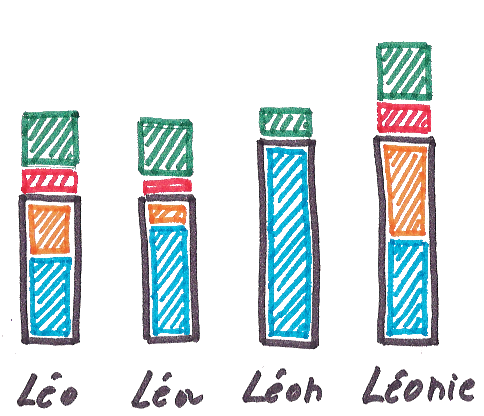
\includegraphics[width=\textwidth]{includes/remuneration}
  \end{center}
  \caption{Notre réponse en image}
  \label{main}
\end{figure}


%Pour nos relecteurs : 
%“Vous serez jugés sur l’originalité, la pertinence, le niveau de détail et la faisabilité du dispositif par une commission (souveraine dans son jugement) composée d’associés et de consultants. Vous pouvez travailler seul ou en équipe (dans ce cas, merci de préciser les noms de l’ensemble des personnes composant le groupe).”
%SAFE (SAlaire Fixe Évolutif) 

\section{Remerciements}

Nous tenons à remercier ANEO pour avoir publié ce concours sans lequel nous n’aurions pas pris le temps de cette mise en commune de nos réflexions. Ces quelques heures passées à échanger sur le sujet ont été une source de satisfaction importante, de prise de conscience et d’idéation maîtrisée. Si c’était à refaire, nous le referions avec grand plaisir. Rendez-vous dans 5 ans, le contexte aura encore évolué et nous pourrons à nouveau nous poser la question. 

Nous tenons aussi à remercier chaleureusement les personnes qui nous ont accordé une denrée rare et même très rare, qu’est leur temps, pour relire ce document et nous permettre d’en faire la meilleure version possible que nous sommes en mesure de faire. Un grand merci à :
\begin{itemize}
  \item Pierre Salanon : l’homme aux convictions qui va nous permettre de faire du développement durable une réalité au-delà du marketing
  \item Michel Chaudy : l’auteur de l’ouvrage “Faire des hommes libres” qui avec sa connaissance de l’économie sociale et solidaire et sa connaissance des communautés de travail de Marcel Barbu a su nous challenger sur 
  \item Ludovic Quesnelle : un manager d’exception qui allie avec finesse autoritarisme et liberté
  \item Céline : pour son pragmatisme
  \item Charles Suire : ancien des communautés de travail pour son regard plein de bienveillance et d’espoir pour nos futures générations pour un monde moins individualistes et plus solidaire
  \item Anne Dupérat : pour ses remarques inspirantes
\end{itemize}


\section{Avant-propos}
\subsection{Pourquoi nous participons à ce concours}
 Ajiro.fr\footnote{\url{http://ajiro.fr}} est un collectif de coach qui cherche à développer des entreprises saines et humaine. Ce sujet, qui nous tient à coeur, vise à remettre l’humain au centre des organisations et à développer le bonheur au travail~\cite{Getz, Laloux}.

 La rémunération est un sujet important dans cette recherche, c’est en effet un élément très visible sur le niveau d’équité, de transparence et de confiance nécessaire à l'épanouissement et à l’engagement de chacun.

 La participation à ce concours nous apparaît donc comme une opportunité de formaliser nos idées sur ce sujet.

\subsection{Rappel de la demande du concours}
 Disponible sur : \url{https://www.linkedin.com/pulse/participez-au-concours-aneo-innovation-sur-la-benoist-debay}

 “ANEO souhaite réfléchir à des modes de rémunération innovants, et plus précisément à la dé-corrélation de l’évaluation annuelle et de la rémunération \cite{Concours}.
 
 Qu’est-ce qui les déclenche, selon quelles modalités, à quelles fréquences... ?
 
 Dans nos typologies d’entreprises, les augmentations/variations de salaire sont dépendantes de notre performance individuelle. Nous « subissons » un entretien individuel qui permet d’évaluer notre performance afin de permettre de nous attribuer un pourcentage d’augmentation. 
 
 Chez ANEO, nous avons la conviction que les évaluations individuelles sont une grande source de stress et ne permettent ni d’améliorer la performance du collectif, ni de nous faire grandir à titre personnel.
 
 Décrivez avec le plus de précisions possibles un processus d’augmentation ne se basant pas sur l’évaluation annuelle.”

\subsection{Notre compréhension de votre demande}
 <<Proposez-nous un système innovant de rémunération des salariés dans un contexte où l’entretien annuel n’existe plus et qui permette de contribuer à un système permettant de grandir à titre individuel et d’améliorer la performance du collectif.>>

 Nous ne traitons dans le cadre de cette proposition ni d’évolution des modes de rémunération ni de la rémunération du capital. Notre proposition présente un fonctionnement en mode cible (tel que nous l’imaginons aujourd’hui). Nous ne présentons pas ici comment passer d’un système de rémunération <<classique>>, <<actuel>> au mode de rémunération cible imaginé.  

\subsection{Définitions}
 Avant de commencer nous souhaitons établir un vocabulaire commun afin de nous accorder sur la signification des mots que nous allons employer.

\subsubsection{Rémunération} 
 La rémunération regroupe un salaire, des avantages, une part variable et une répartition des bénéfices.

\subsubsection{Salaire}
 Selon l’INSEE\footnote{\url{https://www.insee.fr/fr/metadonnees/definition/c1211}} : Le salaire est le paiement du travail convenu entre un salarié et son employeur. 

\subsubsection{Avantage}
 Un ensemble d’éléments payés par l’entreprise, que le salarié peut librement utiliser à titre personnel comme un téléphone portable, une voiture, des livres ou un abonnement ADSL.

\subsubsection{Variable}
 La part variable de la rémunération représente l’ensemble des primes, commissions et la participation aux bénéfices.
 Nous distinguerons par la suite, dans notre proposition, la part variable du salaire et la participation aux bénéfices.

\subsubsection{Persona}
 Selon Wikipedia\footnote{\url{https://fr.wikipedia.org/wiki/Persona\_(marketing)}}, un Persona est une personne fictive qui représente un groupe cible. Lors de la construction du persona, cette personne fictive se voit assigner une série d'attributs qui enrichissent son profil pour mieux exprimer les caractéristiques du groupe cible. Grâce à ces caractéristiques, les équipes de conception (designers) créent des scénarios d'utilisation d'un produit ou d'un service tandis que les équipes commerciales définissent une stratégie de positionnement, de promotion ou de distribution de ce même produit ou service.

\subsection{Conventions typographiques du document}
  Dans la suite du texte, les règles typographiques suivantes seront respectées :

  \assemblee{les éléments laissés à la discrétion de l'entreprise sont identifié dans le reste du texte de cette façon.}

  \actuel{les modes de fonctionnement actuels sont rédigés comme cela dans les texte ci-dessous.}

  \regle{Enfin, les règles applicables à notre modèle de rémunération sont indiquées comme ceci.}

\section{Les systèmes de rémunération actuels}
 Aujourd’hui, la rémunération et l'entretien annuel répondent à un ensemble de besoins allant de la nécessité de faire vivre la famille du salarié à la motivation de ce dernier en passant par la reconnaissance de ses compétences tout en garantissant à ce dernier un plan d’évolution qui s’appuie sur des moments de prise de recul réguliers.

Aujourd’hui la rémunération est un moyen :
 \begin{itemize}
   \item D’exprimer de la reconnaissance (de la valeur, sociale, de l’expérience, de l’investissement de la personne, de la progression de la personne, etc.)
   \item De maintenir la motivation des personnes
   \item De créer l’attractivité de l’entreprise afin d’attirer les talents
 \end{itemize}

Aujourd’hui, les évolutions de rémunération sont soumises à des facteurs de variation tels que :
 \begin{itemize}
   \item La personne ou les personnes en charge de la décision les prennent en toute subjectivité car il s’agit d’un jugement. Et celui-ci peut être fait avec des informations plus ou moins complètes et dans tous les cas teintées d’une interprétation naturelle et peu maîtrisable. Ces personnes en charge de la décision sont aujourd’hui un ensemble restreint d’acteurs de l’entreprise (direction, managers, syndicats, RH, comité de rémunération, clients, etc.).
   \item La capacité de négociation des salariés influe sur le montant de leur rémunération.
 \end{itemize}

L'entretien annuel tel qu’il existe permet de : 
 \begin{itemize}
   \item Prendre du recul sur l’année écoulé : faire un bilan vu du salarié, des collaborateurs, du management, etc.
   \item Mesurer : l’évolution de l’expérience, des compétences, l’adéquation entre la personne et son rôle dans l’entreprise, etc.
   \item Planifier : définir les évolutions dans l’entreprise et les formations ou autres moyens d'accompagnement de cette évolution.
   \item Fixer les objectifs individuels pour l’année à venir. 
 \end{itemize}

 Nous partageons les écueils constatés liés au système actuel.

\section{Notre proposition en quelques mots}
 Nous voyons la rémunération, comme le mécanisme de répartition des risques et des richesses créées par l’entreprise. Dans ce genre de système, il faut souvent prendre des décisions soit égalitaire (tout le monde pareil), soit juste (en fonction des besoins / contributions de chacun). Nous avons fait le choix d’avoir un salaire différencié pour que le système soit juste. En revanche, nous avons décidé de faire une redistribution des bénéfices sur un mode égalitaire. 
 Nous proposons un système de rémunération qui s’appuie sur 3 composantes :
 \begin{itemize}
   \item un salaire fixe défini librement (justice des contributions) 
   \item complété d’une part variable choisie par le salarié (répartition entre variable et fixe défini lors du choix du salaire fixe)
   \item complété d’une répartition des bénéfices fonction du temps de présence dans l’entreprise
 \end{itemize}

 Les grand principes qui ont guidé notre réflexion et dans lesquels nous croyons pour atteindre les enjeux de votre demande à savoir, la progression personnelle et la performance collective, sont :
 \begin{itemize}
   \item Le mécanisme de répartition doit être compris et acceptée par tous les acteurs de l’entreprise pour être volontairement appliqué par l’ensemble des collaborateurs et responsabilisante pour l’ensemble des acteurs de l’entreprise.
   \item Les décisions sont prises par l’ensemble des personnes concernées pour obtenir responsabilisation et liberté de chacun. 
   \item Les informations permettant de prendre les décisions sont disponibles pour tous ceux qui doivent prendre des décisions, c’est la transparence.
   \item Utilisation de la pression sociale pour la régulation des “mercenaires” ou écarts de jugement (sous-estimation ou surestimation)
   \item Suppression totale de la notion de performance individuelle et concentration des efforts sur la création d'une performance collective redistribuée de façon égalitaire sur l'ensemble des salariés 
   \item Possibilité pour les salariés de choisir de partager ou non les risques de l'entreprise fonction de leur situation économique, de leur attrait pour le risque, de leur volonté.
 \end{itemize}

 Dans la définition de notre système nous avons veillé à ce que :
 \begin{itemize}
   \item La rémunération globale soit cohérente avec le marché du travail.
   \item Le système respecte les contraintes fiscales et légales. Le montage précis sera  laissé à la discrétion des comptables et fiscalistes de l’entreprise.
   \item Le système permette la pérennité pour l’entreprise et ses salariés
 \end{itemize}

 Ce dernier point implique 2 axes de réflexions :  
 \begin{itemize}
    \item L’entreprise, la rémunération doit être compatible avec son besoin de trésorerie et d’investissement.
    \item Le salarié, la rémunération doit permettre de vivre sans se poser de question. Une fois les problèmes matériel écartés, il est beaucoup plus facile de s’épanouir dans son travail et d'apporter ainsi un maximum de valeur à l’entreprise.
 \end{itemize}

 Le système que nous proposons ne pourrait remplacer complètement le système actuel sans des briques complémentaires à la rémunération en trois composantes. 

 Ci-après nous décrivons de façon très prescriptive les trois composantes de la rémunération. En effet, c'est le pilier fort du système et le dénaturer pourrait entraîner des dérives du système. 
 
 Pour les autres briques du système (hors rémunération donc), nous décrivons dans la suite du document des exemples de mise en œuvre possible. 

\section{Le système de rémunération}
  \actuel{Dans le système habituel de rémunération, le salarié ne peux pas changer sa rémunération. La régulation des salaires est faite par l’équipe dirigeante.}

 Dans le système que nous proposons, la régulation se fait différemment. 

 Notre proposition vise à réguler les salaires par la transparence et la pression sociale du groupe. La pression sociale s’exercera dans les deux sens, sur-estimation ou sous-estimation de son salaire. 

 A l'extrême, un salarié qui joue contre son entreprise en prenant une rémunération intolérable pour les autres salariés pourrait se voir exclu de l’entreprise. 

 La direction et les RH dans ce mode de fonctionnement basculent sur un rôle d’animation des valeurs et de la vision pour garantir la cohésion du groupe, afin que les décisions individuelles soient cohérentes pour l’organisation. 
 
 Nous pensons en particulier que dans cette situation, les RH doivent pouvoir conseiller et expliquer les rémunérations de chacun, et moins décider.

\subsection{Les trois composantes de la rémunération}
\subsubsection{Le salaire Fixe}

 \regle{Le salaire fixe est libre et défini par chaque salarié sur la base d’une grille de salaire. }

 \assemblee{La grille de salaires est définie par l’ensemble des salariés. Elle pourrait être étayée de persona permettant aux salariés de se comparer et de se situer sur l’échelle et ainsi de se positionner par rapport à un niveau de salaire qu’il estime juste pour lui et pour l’entreprise.}

 La RH (ressources humaines) ou une autre entité (communauté de pairs) pourra aider les salariés à se positionner dans la grille. 
 
 \assemblee{L'entité accompagnant le salarié est à définir par l'ensemble des salariés.}
 
 Un tel système, où le salarié choisit son salaire nécessite de disposer des informations et des outils pour évaluer l’impact sur l’entreprise du choix du salaire ; nous pressentons la nécessité de disposer d’un outil pour faire des simulations pour aider les salariés à prendre les décisions.
 
\begin{figure}
  \begin{center}
  \begin{tabular}{| c | c |}
    \hline
    Niveau & Salaire \\ 
    \hline
    A (option souris) & 1500-1600 \\
    \hline
    B & 2000-2100 \\
    \hline
    C (option chat) & 2500-2600 \\
    \hline
    D & 3000-3100 \\
    \hline
    E (option chimpanzé) & 3500-3600 \\
    \hline
    F & 4000-4100 \\
    \hline
    G & 4500-4600 \\
    \hline
    H & 5000-5100 \\
    \hline
    I & 6000-6100 \\
    \hline
    J & 7000-7100 \\
    \hline
    K & 8000-8100 \\
    \hline
    L (option éléphant) & 9000-9100 \\
    \hline
  \end{tabular}
  \end{center}
  \caption{Exemple de grille de salaires}
  \label{grille}
\end{figure}

\regle{Les éléments clés de l’entreprise (CA - chiffre d’affaire, charges, masse salariales, etc.) qui permettent de prendre des décisions sont rendus publiques également.}

 C’est un élément important de transparence qui permet de réguler les salaires. Cela demande de la pédagogie de la part de la direction ou de l’entité en charge du suivi financier de l’entreprise pour donner cette visibilité et cette conscience au salariés.

 \regle{La position dans la grille de salaire est publique au sein de l’entreprise.}

 Il est fortement conseillé aux salariés de discuter entre eux pour s’harmoniser sur leurs salaires et éviter de mettre en péril l’entreprise\cite{Gore}. Ce sujet est abordé de façon plus détaillée dans le chapitre sur les variations de salaire (cf. section : \ref{sec.variation-salaire}).

 \subsubsection{Le salaire Variable}
 Le variable : le salarié peut choisir de rendre une partie de son salaire fixe variable, pour prendre à sa charge une partie du risque de l’entreprise. En contrepartie, ce variable sera bonifié. 

 Le salarié a la possibilité de choisir une part de variable sur son salaire. Ce dispositif a pour but de prendre en compte une volonté individuelle de participer à la prise de risque. Cela se traduit par le choix d’une répartition du salaire issu de la grille entre salaire fixe versé tous les mois et un variable qui sera reversé à la clôture des comptes. 
 
 %TODO: choose \faUsers or \assemblee
 La réduction du salaire fixe versé mensuellement permet à l’entreprise de disposer de plus de liquidités. Lors de la redistribution des bénéfices en fin d’exercice, les personnes qui ont fait le choix de cette prise de risque sont “remboursées” en priorité ; ce “prêt” à l’entreprise est bonifié par un coefficient multiplicateur qui sera défini par l’ensemble des salariés \faUsers. Dans le cas où les bénéfices de l’entreprise ne permettent pas de couvrir les variables volontaires bonifiés, une répartition sera faite au prorata de la part de salaire “prêté” par le salarié à l’entreprise.

\subsubsection{La redistribution des bénéfices}
\actuel{Aujourd’hui le variable est indexé sur l‘atteinte d’objectifs individuels. Ce système favorise la compétition puisqu’à enveloppe de redistribution égale, celui qui en aura le plus est celui qui pourra justifier de l’atteinte la plus proche de ses objectifs. Cette évaluation étant subjective, il s'ensuit un jeu de séduction et de compétition (parfois inconsciemment) pour être celui qui brille le plus auprès de ceux qui vont prendre les décisions.}

\regle{La redistribution des bénéfices se fait de façon égalitaire au prorata temporis.}
 
 En fin d’exercice, l’entreprise définie, explique et publie la répartition des bénéfices de l’entreprise entre :
 \begin{itemize}
   \item Les investissements
   \item La trésorerie
   \item La rémunération du capital
   \item La redistribution des bénéfices
 \end{itemize}

 C’est pourquoi dans notre système nous attachons autant d’importance au fait de ne pas découper la performance collective en éléments de performance individuelle ou d'objectifs. Pour rappel, notre vision du système cible est un système à la fois juste et égalitaire. Le salaire fixe permet d’apporter la justice car le salarié choisit un salaire cohérent avec sa contribution. 

 Notre proposition est de redistribuer les bénéfices au prorata temporis des salariés, sous une forme compatible avec la législation et la fiscalité (participation aux bénéfices, primes, PEE, etc.).  Ainsi plus l'entreprise au global fait de bénéfices et plus chaque salarié bénéficiera d'une rémunération importante puisque sa part de bénéfice sera plus importante. Cette proposition doit permettre de favoriser l’engagement collectif, l’entraide et limiter les combats d’ego au bénéfice du collectif : On passe du “toi OU moi”, au “toi ET moi”. “Si tu gagnes, je gagne” au lieu de “si tu gagnes, je perds”.

\subsection{Exemple}

 \begin{center}
 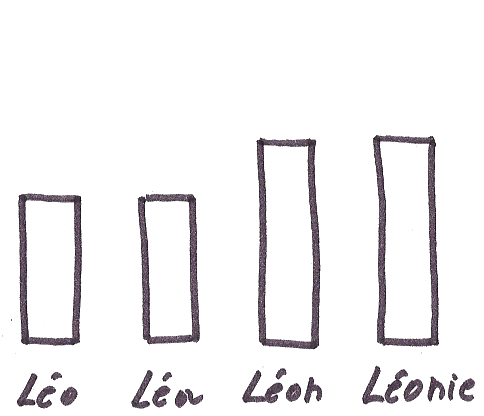
\includegraphics[width=0.6\textwidth]{includes/choix_salaires}
 \end{center}

 Aujourd'hui, c'est la grande réunion de la rémunération, Léo, Léa et Léonie ont tous les 3 choisis leur salaire dans la grille. Léon arrivera en cours d’année son salaire sera négocié dans la grille, il est déjà représenté sur l'illustration.

 \begin{center}
 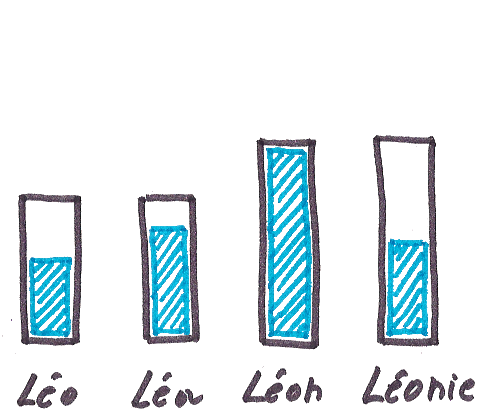
\includegraphics[width=0.6\textwidth]{includes/choix_part_fixe}
 \end{center}

 Léo a choisi de ne recevoir tous les mois que 60\% de son salaire, Léonie a fait le choix de ne recevoir que 50\% de son salaire. Ils laissent le reste dans l’entreprise pour en partager les risques.

 Léa a un plus grand besoins de liquidité dans son couple, elle vient d’avoir un bébé. Elle a donc choisi de prendre 80\% de son salaire sous forme fixe.

 \begin{center}
 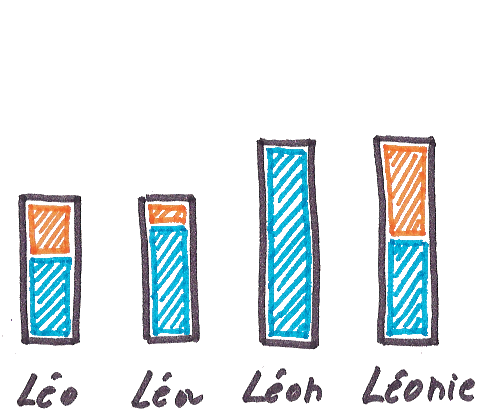
\includegraphics[width=0.6\textwidth]{includes/choix_part_variable}
 \end{center}

 C’est la fin de l’année, le moment de faire le bilan financier. La société a fait une très bonne année, elle peut donc verser à nos 4 amis la totalité de leur part variable.

 \begin{center}
 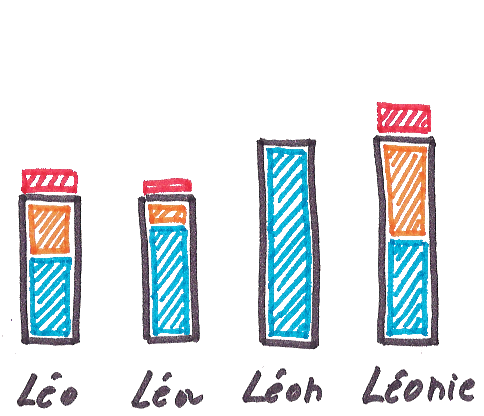
\includegraphics[width=0.6\textwidth]{includes/versement_bonification}
 \end{center}

 Accompagné de la bonification correspondante.

 \begin{center}
 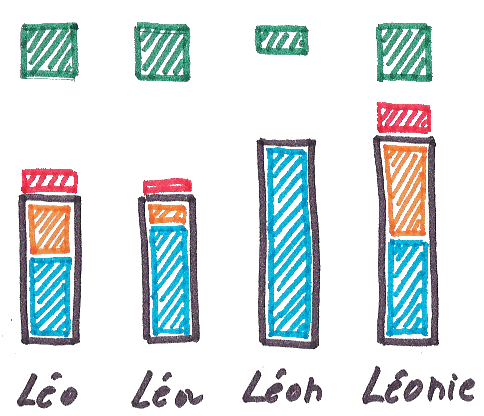
\includegraphics[width=0.6\textwidth]{includes/versement_benefices}
 \end{center}

 Les résultats sont tellement bon, qu’il reste de quoi verser une participation aux bénéfices. Léon n’étant là que depuis 6 mois, il n’a que la moitié de cette participation.

 \begin{center}
 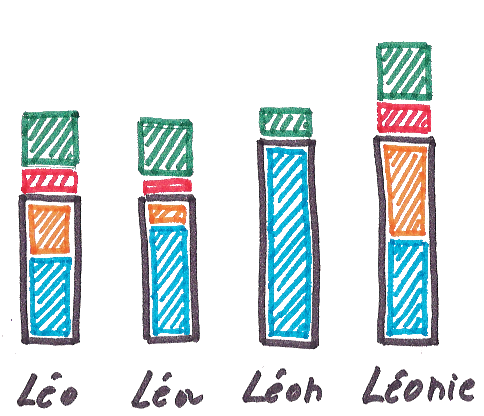
\includegraphics[width=0.6\textwidth]{includes/remuneration}
 \end{center}
 Au final voici les rémunération annuel de nos quatres amis.

\subsection{Les variations de salaire}
\label{sec.variation-salaire}
 Les variations de salaire sont de plusieurs natures : 
 \begin{itemize}
   \item Soit systématiques.
   \item Soit à l’initiative du salarié.
 \end{itemize}

 \vspace{3mm}
 \regle{Systématique : le salaire suit le coût de la vie ; la grille évolue avec l’inflation.}

 Tous les ans la grille des salaires peut être réévaluée en fonction de l’inflation définie par l’INSEE.

 \regle{A l'initiative de chaque salarié : il peut demander à changer de salaire quand il le juge nécessaire, à la hausse ou à la baisse.}

 Les principes de transparence et donc de pression sociale restent applicables. Ainsi comme précédemment, les RH peuvent être des partenaires de réflexion dans le choix du nouveau salaire. Leur intervention est complémentaire des échanges entre salariés. Nous encourageons donc les salariés à discuter des modifications de salaire entre eux pour s’harmoniser. 

 Point important, la transparence est réalisée en mode poussé : les modifications de salaires sont notifiées à l’ensemble des salariés. 

 \assemblee{L’ensemble des salariés peut définir des modalités plus précise de revue des salaires. }
 Voici quelques exemples :
 \begin{itemize}
   \item Les revues de salaire seront réalisées par chacun et un système de revue par les autres salariés est organisé (la possibilité de donner un avis, via un outil par exemple).
   \item Les revues de salaire seront réalisées par chacun à des périodes clés définies. 
   \item Les revues de salaires seront toutes réalisées sur les mêmes périodes à la fréquence définie.
   \item Des journées annuelles de revues des rémunérations regrouperaient tous les acteurs et permettraient de parcourir en groupe le processus de réévaluation pour le bénéfice de l'ensemble du groupe.
 \end{itemize}

\subsection{L’embauche et l’intégration}

 Notre système décrit également les modalités d’intégration d’un nouveau salarié venant d’un environnement où le système serait différent.

 L’embauche d’un nouveau salarié se fera en utilisant la grille de salaire et négocié durant le processus de recrutement, comme d’habitude. 

 Le système de rémunération cible décrit ici ne sera applicable qu’après une certaine période que nous appelons le “postulat”. Cette période de “postulat” est une période d’acculturation du nouvel embauché à la culture de l’entreprise. Elle doit entre autre lui permettre de comprendre comment fonctionne le système de rémunération pour lui permettre de jouer avec les mêmes règles du jeu en toute connaissance de causes. Ici l’hypothèse est que la durée de postulat dure 12 mois. 

 \assemblee{La durée de ce postulat peut être soumise à une approbation de l’ensemble des acteurs de l’entreprise.}

 Le nouvel arrivant intègre l’entreprise en tant que “postulant” et conserve son salaire d’embauche pendant un an, le temps de comprendre le mode de fonctionnement et d’acquérir les éléments de référence lui permettant de se positionner dans la culture.  

 Nous pensons qu’il serait utile qu’un nouvel embauché soit parrainé pendant cette période par un salarié pour donner des clés de lecture sur le fonctionnement de l’entreprise.

 Lors des échanges précédents l’embauche, l’explication de la rémunération suite à leur période de “postulat” peut être un élément d’attrait de nouveaux collaborateurs. 

\section{Les autres briques du système}

 Notre proposition concernant la rémunération s’arrête ici. 

 Cependant, le système que nous vous proposons ne peut fonctionner si les besoins couverts par le système “classique” de rémunération n’est pas couvert par un autre dispositif. Dans la suite du document nous proposons quelques modalités de mise en oeuvre afin de vous permettre d’imaginer à quoi le système complet pourrait ressembler. Le niveau de description des modalités suivantes restera donc assez macroscopique.

\subsection{Attirer de nouveaux talents}

 Attirer les talents pourra se faire sur les même critères que ceux de la motivation. Il est en effet dangereux, pour nous, d’attirer les talents avec une rémunération alléchante car cela attire des mercenaires qui ne partagent souvent ni les valeurs ni la vision de l’entreprise.

\subsection{La motivation}

 Aujourd’hui le système s’appuie sur une prime obtenue sur atteinte d’objectifs individuels annuels. 

 Nous pensons que l’argent n’est que rarement une source de motivation. Cela peut être une source de démotivation quand le salaire est insuffisant pour couvrir les charges de la personne ou que les critères de répartitions sont ressentis comme injustes. Notre proposition de rémunération n’est donc pas basée sur cette croyance que l’argent implique la motivation. 

 Nous pensons que la motivation des salariés peut jouer sur d’autres leviers. Ci-dessous quelques exemples :
 \begin{itemize}
   \item L’image de l’entreprise et sa notoriété pour pouvoir dire avec fierté : « Je travaille chez Spotify » au lieu de « je suis CEO et j’ai une voiture de fonction ».
   \item Le cadre de travail (espaces de travail “sympa”, label “great place to work”, Gallup Q12, baromètre de motivation des équipes, etc.).
   \item L’autonomie et les responsabilités que l’on peut exercer.
   \item Les apprentissages que l’on peut explorer (technologiques, humain, etc.).
   \item Les conférences et autres événements auxquelles on peut participer.
   \item Les sujets sur lesquels on travaille (innovations, passions).
   \item L’appartenance à des communautés internes.
   \item Les relations que l’on a avec ses collègues (managers ou pas).
   \item La possibilité de faire entendre sa voix en optant pour des modes d’organisation où tous ceux qui veulent s’exprimer en ont l’opportunité (holacratie\footnote{\url{https://fr.wikipedia.org/wiki/Holacratie}}, sociocratie\footnote{\url{https://fr.wikipedia.org/wiki/Sociocratie}}, etc.).
   \item Créer des espaces de discussion en face à face réguliers pour des sujets personnels en laissant au salarié le choix de son partenaire.
   \item Créer des espaces d’échanges en groupe pour des sujets personnels, de montée en compétences ou pour les décisions qui impactent toute l’entreprise.
   \item L’équité dans le traitement : que les règles soient claires et appliquées de la même façon par tous. Certaines organisations disposent de commission de discipline qui est chargé de résoudre avec le salarié et un groupe de pairs un écart aux règles convenues.
 \end{itemize}

\subsection{La reconnaissance}
 \actuel{Aujourd’hui, la reconnaissance sociale peut passer par la représentation d’un statut dans l’entreprise et par des avantages en nature associés : “Je suis manager et j’ai une voiture de fonction”.}

 Dans une entreprise plus libérée, ce genre de médaille n’a plus lieu d’être. La reconnaissance vient directement de la satisfaction à participer à la réussite de l’entreprise. Liberté et confiance en soi permettent de transcender ces signes extérieurs. 

 Nous pensons que la reconnaissance sociale peut évoluer vers une reconnaissance liée à l’appartenance à une société  (ex : je travaille chez Google, Favi, etc.)

 Les autres types de reconnaissance telles que la reconnaissance de l’expérience de la personne, de l’investissement de la personne, de la progression de la personne, etc. sont traités dans la prise de recul ci-dessous. 

 Être responsable et devenir autonome en respectant la ligne de flottaison (et donc ne pas mettre en risque l’entreprise) c’est être capable de prendre des décisions en connaissance de cause, en connaissant ses propres limites et celles des autres. Cela signifie être en mesure de reconnaître ce que chacun apporte, les autres autant que soi. Pour pouvoir évaluer ces apports, la prise de recul régulière suivants plusieurs axes est nécessaire. Et pour que ces prises de conscience soit partagées, savoir recevoir et donner du feedback est important. C’est un élément de culture dont le système aura besoin pour se pérenniser.

\subsection{La prise de recul}

 Aujourd’hui réalisée lors de l’entretien annuel, la prise de recul est un bilan régulier réalisé par le salarié ou des collaborateurs (360\degre) ou le management direct afin de mesurer les évolutions en termes d’expérience, de compétences, d’évaluer l’adéquation entre la personne et son rôle dans l’entreprise, etc.

 Nous préconisons de faire des prises de recul de façon plus fréquente et tout aussi régulière. Il s’agit alors de proposer au salarié différents dispositifs. Charge au salarié ensuite de prendre ses responsabilités et d’utiliser celles qui lui conviennent le mieux au service de la couverture de ses besoins et de son épanouissement. 

 Ci-dessous quelques exemples possibles de modalités de mise en oeuvre liées à la prise de recul :
 \begin{itemize}
   \item Auto-évaluation régulière par le salarié (en accompagnement ou seul)
   \item Échanges avec un binôme de confiance choisi par le salarié
   \item Faire partie de communautés de pratiques au cours desquelles des sessions de co-développement professionnel peuvent être réalisées
   \item Réaliser des séances de supervision
   \item Faire des 360\degre incluant les clients
   \item Mettre en place un système de recommandation interne / externe de ses collègues que le salarié peut activer chaque fois qu’il a pu constater par l’expérience une compétence avérée chez son collègue
   \item Mettre en place des rituels de célébration de réussites de l’entreprise
   \item Mettre en place des rituels d’apprentissage d’entreprise.
 \end{itemize}

 Remarque importante : les actions ci-dessus n’ont pas de périodicité, elles peuvent avoir lieux quand le salarié le décide. Il reprend ainsi la maîtrise de son rythme d’évolution et du sens de son évolution.

 La RH et le management sont au service des salariés pour proposer, aider à choisir, échanger. 

\subsection{L’évolution du collaborateur}
 \actuel{Aujourd’hui, lors de l’entretien annuel, des formations, coaching et autres parcours initiatiques sont définis pour accompagner le salarié dans son développement au service de l’atteinte de ses objectifs annuels.}

 Dans notre système, la responsabilité de son évolution est rendue au salarié. L’entreprise lui met à disposition un ensemble de dispositifs que le salarié peut décider d’activer ou non en fonction de ses besoins. Ces dispositifs lui permettent de définir ses prochains challenges, d’identifier les formations ou autres moyens d'accompagnement qui lui seront nécessaires pour sa progression.

 Voici quelques exemples de dispositifs que l’on peut proposer aux salariés et qu’ils peuvent choisir d’utiliser, d’activer si et quand ils le souhaitent :
 \begin{itemize}
   \item Réaliser des entretiens avec des mentors internes ou externes à l’entreprise
   \item Faire intervenir des personnes extérieures pour témoigner des évolutions du marché, pour inspirer de nouvelles envies d’évolution, pour ouvrir de nouvelles perspectives
   \item Animer des sessions de remise en question de l’entreprise et de projection avec ses clients
   \item Participer au marketing de la société pour sentir de plus prêt les évolutions du marché (conférences, colloques, démarchage de prospects, etc.)
   \item Mettre en place un groupe de travail pour réfléchir et définir les formations stratégiques pour l’entreprise
   \item Mettre en place un budget de formation pour chaque collaborateur (comme les abonnements téléphoniques, avec report de forfait).
 \end{itemize}

\subsection{Les attentes des salariés vis-à-vis des entités RH et du management }

 Le système décrit montre que les attentes des salariés par rapport aux fonctions managériales et aux fonctions support seront différentes de celles qui existent aujourd’hui. Le salarié reprenant le pouvoir de décision et étant prêt à partager les risques et bénéfices de l’entreprise, ce qu’il va attendre de ces entités sera essentiellement : 
  \begin{itemize}
    \item De la transparence et de la pédagogie (explication de la grille, des persona, du mode de fonctionnement, de l’adéquation salaire/personne, etc.)
    \item De l’accompagnement dans la réflexion et le choix pour le bien du salarié et de l’entreprise (définition de dispositifs de prise de recul, aide dans le choix des évolutions de carrière possibles, dans les choix d’outils de progression, échange sur les envies, mise en perspective, etc.)
  \end{itemize}

 Ainsi, la direction et les RH dans ce mode de fonctionnement basculent vers un rôle d’animation des valeurs et de la vision pour garantir la cohésion du groupe, afin que les décisions individuelles soient cohérentes pour l’organisation. 

 D’autre part, nous pensons qu’il faut être vigilant et accompagner de façon plus attentive les salariés ayant une faible estime de soi et qui pourraient se retrouver en difficulté.

\nocite{*}
\printbibliography

\end{document}

